
\documentclass[10pt,journal,compsoc]{styles/IEEEtran}
\usepackage{styles/algorithm}
\usepackage[noend]{styles/algorithmic}
\usepackage{graphicx}
\usepackage{color}
\usepackage{listings}
\usepackage{amsmath}
\usepackage[utf8]{inputenc}
\usepackage[T1]{fontenc}
\usepackage[labelformat=empty]{caption}
% *** CITATION PACKAGES ***
\ifCLASSOPTIONcompsoc
  % IEEE Computer Society needs nocompress option
  % requires cite.sty v4.0 or later (November 2003)
  \usepackage[noadjust]{cite}
\else
  % normal IEEE
  \usepackage{cite}
\fi

\title{Tarea 3: M\'ETODO DE REGI\'ON DE CONFIANZA}

\author{Juan Gerardo Fuentes Almeida}

% The paper headers
\markboth{Tarea 3:M\'ETODO DE REGI\'ON DE CONFIANZA }%
{Shell \MakeLowercase{\textit{et al.}}: Bare Advanced Demo of styles/IEEEtran.cls for Journals}

\IEEEtitleabstractindextext{%
\begin{abstract}
En esta pr\'actica se implementa el algoritmo de Regi\'on de Confianza al problema de registro r\'igido de im\'agenes.
\end{abstract}
}

\begin{document}

% make the title area
\maketitle

\IEEEdisplaynontitleabstractindextext

\IEEEpeerreviewmaketitle

\section{Introducci\'on}

\IEEEPARstart{L}os M\'etodos de la Regi\'on de Confianza constituyen una metodolog\'ia reciente en optimizaci\'on, se basan en un problema de aproximaci\'on m\'as que en una direcci\'on.\\

Se construye una funci\'on modelo $m_k(x)$ cuyo comportamiento cerca de la iteraci\'on actual $x_k$ es similar a la funci\'on obetivo $f$, por esta raz\'on se le llama m\'etodo de Regi\'on de Confianza.\\

Como el modelo $m_k$ puede no ser una buena aproximaci\'on de $f$ cuando $x$ esta lejos de $x_k$, se restringe la b\'usqueda de un \'optimo de $m_k$ en alguna regi\'on en torno a $x_k$.\\

Si la soluci\'on candidata no produce un decrecimiento suficiente en $f$ se concluye
que la regi\'on de confianza es demasiado grande y debe reducirse para despu\'es resolver el subproblema asociado.\\


\section{Teor\'ia}

\subsection{Regi\'on  De Confianza }

El modelo en un m\'etodo de regi\'on de confianza est\'a usualmente definido por una
funci\'on cuadr\'atica de la forma:\\

$m_k(x_k+p)=f(x_k)+p^T \nabla f(x_k)+\frac{1}{2}p^T B_k p$\\

donde la matriz $B_X$ es, o bien el Hessiano $\nabla^2f(x_k)$ o alguna aproximaci\'on de
\'este.\\

Si $B_x$ =0 y se define la regi\'on de confianza como la una norma Eucl\'idea, el problema de regi\'on de confianza se resume en:\\

$min f(x_k)+p^T\nabla f(x_k)$ sujeto a $\alpha\|p\|\leq\Delta_k$\\

Un algoritmo de regi\'on de confianza m\'as interesante se obtiene eligiendo $B_K$ como el hessiano $\nabla^2f(x_k)$ en el modelo cuadr\'atico. Como se tiene la restricci\'on
de la regi\'on de confianza $\alpha\|p\|\leq\Delta_k$ no es necesario que $\nabla^2f(x_k)$ sea definido positivo pues se tiene asegurada la existencia de una soluci\'on $p_k$.\\

El tama\~no de la regi\'on de confianza es cr\'itico para la eficacia de cada paso. Si la
región de confianza es muy  peque\~na ,el algoritmo pierde la oportunidad de dar
un paso importante para desplazarse cerca del minimizador de la función objetivo $f$.\\

\begin{figure}[hbtp]
\centering
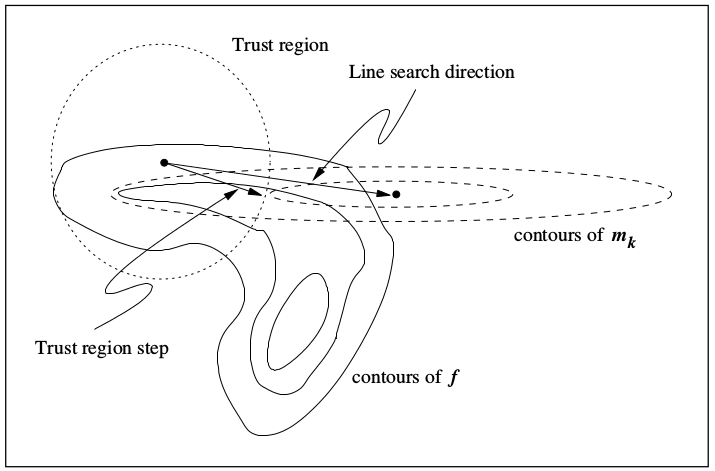
\includegraphics[width=0.45\textwidth]{mrc.png}
\caption{B\'usqueda en L\'inea vs Regi\'on de Confianza}
\end{figure}

Por otro lado, si es muy grande, el minimizador del problema puede estar lejos del minimizador
de la funci\'on objetivo en la regi\'on, dando como resultado un avance no deseado, una soluci\'on para \'esta situaci\'on ser\'ia reducir el tamaño de la regi\'on de confianza,
e intentar resolver nuevamente.\\

En consecuencia a lo anterior se tiene que la elecci\'on de $\Delta_k$ debe basarse en la funci\'on f mediante la funci\'on $m_k$ empleando el siguiente par\'ametro . \\

$\rho_k =\frac{f(x_k)-f(x_k+p_k}{m_k(0)-m_k(p_k)}$\\

donde $p_k$ es un paso a partir de la iteraci\'on actual $x_k$ .
Al numerador se le llama reducci\'on actual y al denominador reducci\'on prevista.

Debemos notar  que como el paso $p_k$ lo podemos obtener  minimizando el modelo $m_k$
en una regi\'on que incluye $p = 0$ , tomando en cuenta que la reducci\'on prevista ser\'a siempre no negativa, entonces si $\rho_k$ es negativo el nuevo valor objetivo $f(x_k+p_k)$ es mayor que el valor actual $f(x_k)$ por lo que el paso debe ser rechazado.\\

\begin{figure}[hbtp]
\centering
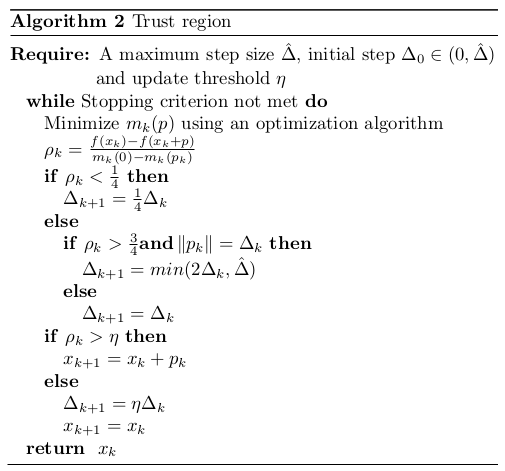
\includegraphics[width=0.45\textwidth]{TrustRegion.png}
\caption{}
\end{figure}


\subsection{Algoritmo de Dog-Leg}

El algoritmo de Dog-Leg se basa en el c\'alculo del Punto de Cauchy, es el reductor de $m_k$ a lo largo de la direcci\'on de m\'aximo descenso $g_k$  sujeto a la regi\'on de confianza. No es necesariamente un minizador del modelo, pero si aporta un suficiente descenso dentro de la region de confianza\\

Este m\'etodo utiliza el c\'alculo tanto de la direcci\'on de Newton de descenso, as\'i como la direcci\'on de descenso de gradiente y el radio de la region de confianza para encontrar una $p_k$ \'optima que produzca un suficiente descenso.

\begin{figure}[hbtp]
\centering
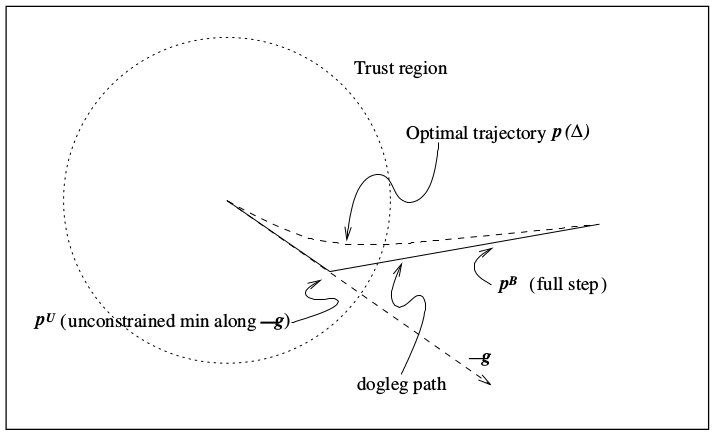
\includegraphics[width=0.45\textwidth]{dogleggraph.png}
\caption{M\'etodo de DogLeg}
\end{figure}
 

 \begin{figure}[hbtp]
\centering
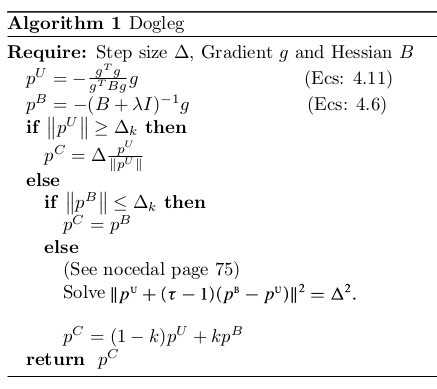
\includegraphics[width=0.45\textwidth]{dogleg.png}
\caption{}
\end{figure}
 
 
\section{Resultados}

Como parte de la pr\'actica, se tom\'o un conjunto de im\'agenes de resonancia magn\'etica para implementar un registro r\'igido y minimizar la funci\'on de error determinada por la siguiente expresi\'on:\\

\begin{figure}[hbtp]
\centering
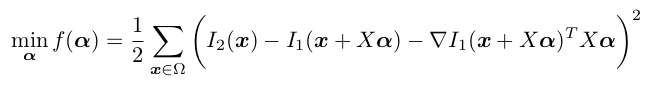
\includegraphics[width=0.45\textwidth]{error.png}
\caption*{}
\end{figure}

$I_2$ es una imagen de referencia, $I_1$ es la imagen observada cuyo dominio est\'a definido en $x={x_1,x_2}$, de manera que $\omega$ representa el conjunto de todos los pixeles de la imagen, $X$ y $\alpha$ son variables definidas de la siguiente manera:\\

\begin{figure}[hbtp]
\centering
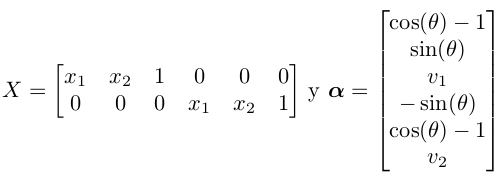
\includegraphics[width=0.45\textwidth]{variable.png}
\caption*{}
\end{figure}

Esto permite que la transformaci\'on de una imagen a otra este dada por el producto $x+X\alpha$\\


\begin{figure}[hbtp]
\centering
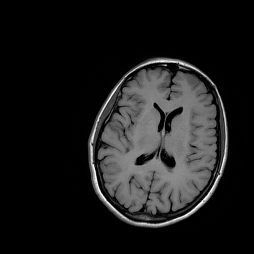
\includegraphics[width=0.35\textwidth]{mriC.png}
\caption{Imagen Inicial u Observada}
\end{figure}

\begin{figure}[hbtp]
\centering
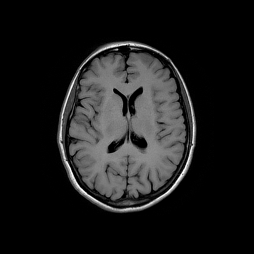
\includegraphics[width=0.35\textwidth]{mriReferencia.png}
\caption{Imagen de referencia}
\end{figure}

El gradiente y el Hessiano de esta funci\'on est\'an definidos de la siguiente manera:\\

$\nabla f(\alpha)=\Sigma[I_2(x)-I_1(x)][-X^T \nabla I_1(x+X\alpha)]$\\
$\nabla^2 f(\alpha)=\Sigma[X^T \nabla I_1(x+X\alpha)][X^T \nabla I_1(x+X\alpha)]^T$\\

En la pr\'actica, estas funciones fueron las que nos dieron mejores resultados.\\

El algoritmo lee los archivos de las dos im\'agenes y realiza la minimizaci\'on de la funci\'on objetivo con el m\'etodo de la Regi\'on de Confianza, en conjunto con el m\'etodo de Dogleg para el c\'alculo del punto de Cauchy; se inicia con un desplazamiento inicial de 10 pixeles hacia arriba y hacia la izquierda para acercarnos un poco a la posici\'on de la imagen de referencia.

\begin{figure}[hbtp]
\centering
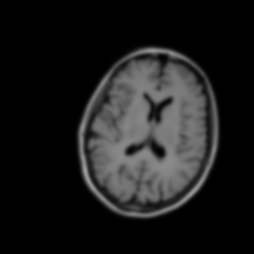
\includegraphics[width=0.35\textwidth]{mriCinicial.png}
\caption{Imagen inicial, se tuvo que hacer un emborronado de la imagen para obtener mejores resultados}
\end{figure}

\begin{figure}[hbtp]
\centering
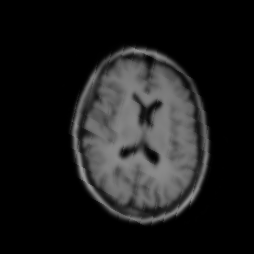
\includegraphics[width=0.35\textwidth]{mriCfinal.png}
\caption{Imagen final despues de 20 mejoras, se aprecia la rotacion que se produce para empalmarse con la imagen de referencia}
\end{figure}

Aunque la funci\'on objetivo siempre muestra valores demasiado grandes, se pudo observar una mejor\'ia en la posici\'on y orientaci\'on de la imagen con respecto a la de referencia. Otro comportamiento observado fue que a partir de cierto n\'umero de iteraciones, la funci\'on objetivo deja de disminuir qued\'andose en un valor muy grande y reduciendo pr\'acticamente a cero la regi\'on de confianza.


\section{Conclusiones}

En general no se obtuvieron los resultados que se esperaban, se tuvieron muchos problemas, principalmente con repecto a la correcta definici\'on de la funci\'on objetivo y sus derivadas, tambi\'en se tuvieron problemas con los m\'etodos de optimizaci\'on vistos en clase, los cuales directamente aplicados a este problema no produc\'ian los resultados esperados. Se espera que en futuras pr\'acticas se afinen m\'as detalles sobre este tipo de implementaciones.

\bibliographystyle{plain}
\bibliography{biblio}


\appendix
\section{Implementation details}
El programa est\'a implementado tomando en cuenta todas estandarizaciones indicadas en el curso.

Un \textit{makefile} ha sido generado, el cual soporta los comandos \textit{make}, \textit{run} and \textit{clean}. El programa recibe como primer argumento el nombre del archivo de la imagen inicial, y como segundo argumento el nombre del archivo de la imagen de referencia.


\end{document}


